\section{FSMDriver}\label{sec:3}%
Driving a car can be intuitively divided into several behaviors, and thus provide a straightforward implementation as a finite-state machine model. Such model's configuration parameters can be optimized through a genetic algorithm, and the TORCS/SCR platform provides a standard measure of driver quality, and its sensor/actuator interface enable it to be readily replaced by actual robotic prototypes (or other more advanced models) for further testing. This work proposes to use these ideas for evolving a controller for a car, the FSMDriver, as one more step towards autonomous vehicles.

\newcommand{\state}[1]{\texttt{#1}}%
\newcommand{\SL}{\state{Straight Line}}%
\newcommand{\C}{\state{Curve}}%
\newcommand{\OT}{\state{Out of Track}}%
\newcommand{\St}{\state{Stuck}}%
\newcommand{\AC}{\state{Approaching Curve}}%
\newcommand{\IT}{\state{Inside Track}}%

\subsection{Driving Behaviors}%
A \state{State} in the FSM model considered here defines a racing behavior, deciding the driver's output according to the given sensor input as defined by SCR's API. The FSM implements a transition function that, at every game tick, analyses the input and decides which state is appropriate, triggering a change if necessary. The state then processes the input and defines the proper output.

The next step for implementing the FSM model is defining its states. Intuitively, \state{Driving}~could be a definite solution but it obviously involves several distinct situations which should be divided, simplifying the development.

Considering the testing environment, it is clear that two antagonistic situations that require specific behaviors: \state{Racing}, for situations where the car is within track limits, facing the right direction; and \state{Recovery}, for when the car is outside track limits or facing the right direction, or unable to move.

These can be further divided into two more specific behaviors for implementation:
\begin{description}
	\item[\SL:] for racing straight ahead;
	\item[\C:] for racing through a curve;
	\item[\OT:] for recovering from leaving the track or facing the wrong direction; and
	\item[\St:] for recovering from being unable to move forward.
\end{description}

Each of these states implements its behavior as follows. \SL~ attempts to go as fast as possible parallel to the track axis by accelerating at full throttle, which improve the performance to track's variance, and changing gears according to RPM thresholds. \C~steers towards the direction towards the track sensor with the largest reading (see Figure~\ref{Fig:FSensor}) with 60\% throttle, since it indicates at each state iteration a retiline path to exit the curve, braking in case it starts to slide in the X axis. \OT~ attempts to return to the track, facing the right direction, adjusting its speed and steering according to its current orientation concerning the track (see Figure~\ref{Fig:Angle}). \St~ tries to get unstuck by using the reverse gear and hard steering.

\begin{figure}[h]
	\centering
	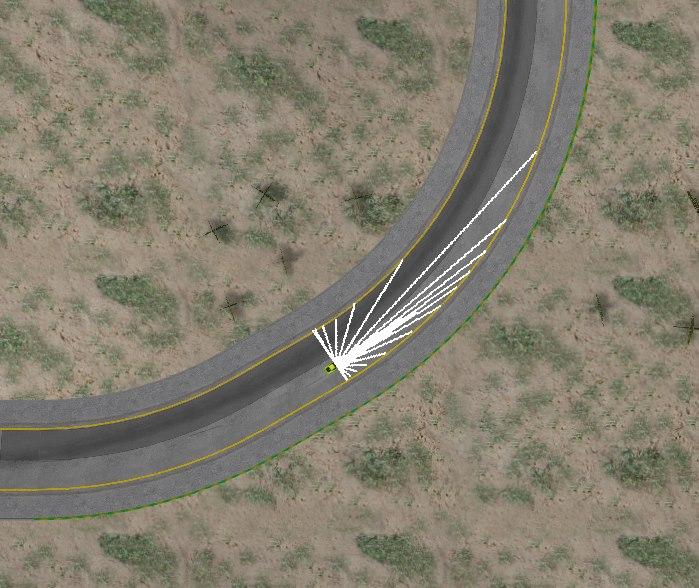
\includegraphics[width=250pt]{FarthestSensor}
	\caption{Sensor input in curve.}
	\label{Fig:FSensor}
\end{figure}

\begin{figure}%[h]
		\centering
		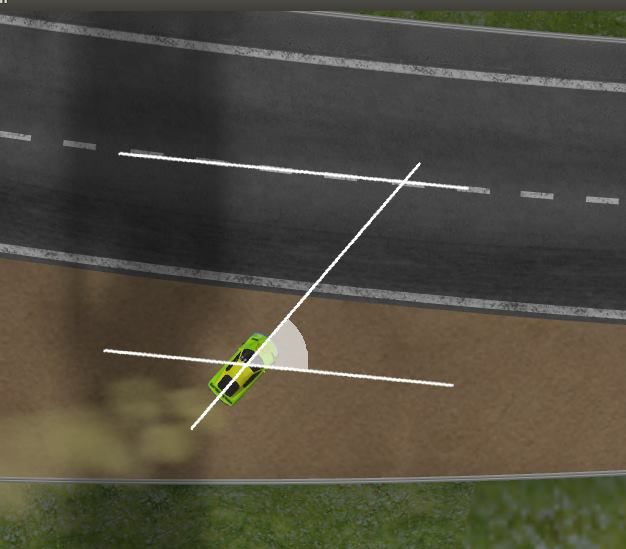
\includegraphics[width=250pt]{ReturnAngle}
		\caption{Angle between car and track axis.}
		\label{Fig:Angle}
\end{figure}

\subsection{FSMDriver5}

Initial tests showed that transitioning from \SL~to \C~was too swift, hampering performance because the car consistently entered curves at such high speeds that the controller was unable to turn and exited the track, so the additional behavior \AC~was implemented. \AC~positions the driver towards the outside of the incoming curve and tries to race at a speed proportional to the curvature, so less braking would be necessary in \C. Thus, a 5-state FSMDriver (FSMDriver5) model (illustrated in Figure~\ref{Fig:FSM5Diagram}) was ready for testing.

\begin{figure}[h]
	\centering
	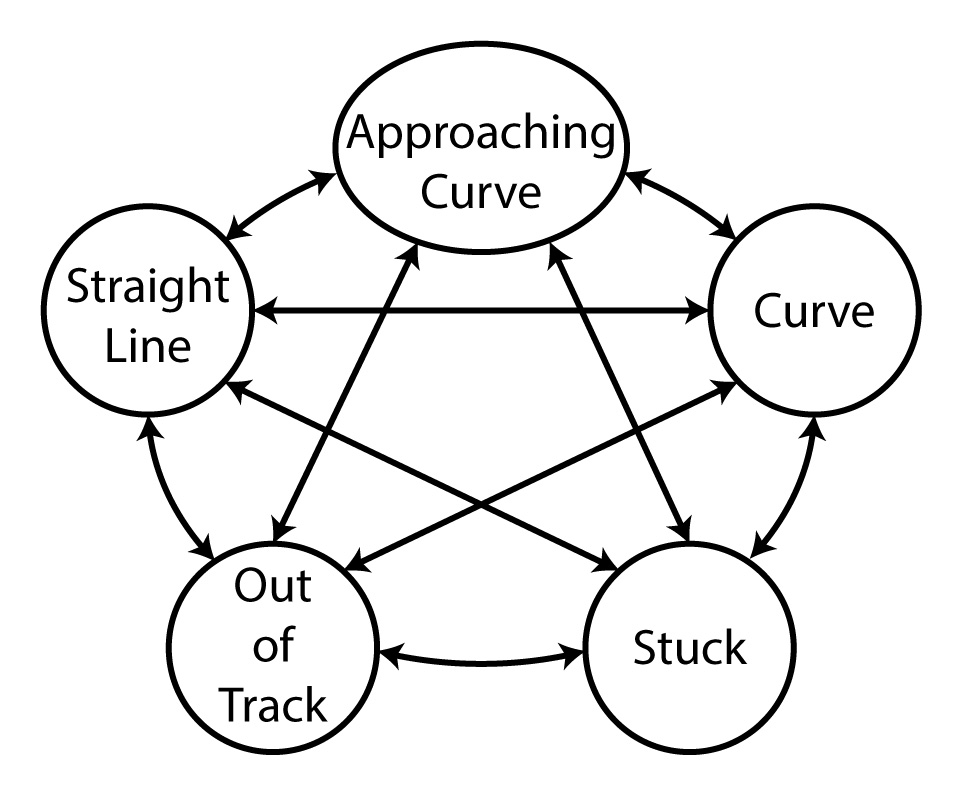
\includegraphics[width=.45\textwidth]{FiveStateFSM}
	\caption{FSMDriver5 state diagram.}
	\label{Fig:FSM5Diagram}
\end{figure}


There are 19 range finders available in SCR~\cite{SCR} whose directions are defined by the driver, and these sensors provide the distance between the car axis and the edge of the track. When the car is outside of the track's boundaries, they read $-1$ value. For the Five-State driver, those directions were arbitrarily settled from $-90$ to $90$ degrees in a $10$ degree step, the $0$ degree direction pointing toward the car axis, see Figure~\ref{Fig:FSM5Sensors}.

\begin{figure}[h]
	\centering
	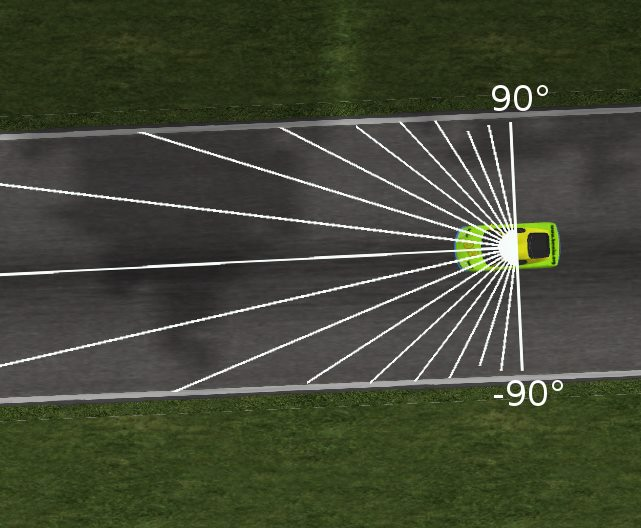
\includegraphics[width=250pt]{FSM5Sensors}
	\caption{FSMDriver5 range finders.}
	\label{Fig:FSM5Sensors}
\end{figure}

Through several observations it was concluded that the farther from a curve the car is, the greater the difference among the frontal and lateral sensors is. As the car approaches a turn this difference starts to drop until it reaches a minimum value, when the car is taking the turn. The variance among the range finders was taken into account for telling which state of the \state{Racing} behavior would better fit with the current segment of the track, as shown in Algorithm \ref{alg:FSMDriver5}.


\begin{algorithm}[h]%
\caption{FSMDriver5 Transition}%
\label{alg:FSMDriver5}%
\begin{algorithmic}
    \IF{car is stuck}
        \STATE $state \Leftarrow Stuck$
    \ELSE
	\IF{($variance < MAX\_STRAIGHTLINE\_VAR$) \OR ($variance < MIN\_STRAIGHTLINE\_VAR$ \AND
   	the current state is not $StraightLine$)}
   		\STATE $state \Leftarrow StraightLine$
	\ENDIF
	\ELSIF{($variance >MAX\_APPROACHING\_CURVE\_VAR$ \AND current state is not curve)
         \OR ($variance > MIN\_APPROACHING\_CURVE\_VAR$ \AND current state is not Approaching Curve)}
		\STATE $state \Leftarrow Approaching Curve$
	\ELSIF{$variance>0$}
		\STATE $state \Leftarrow Curve$
	\ELSE
		\STATE $state \Leftarrow Out Of Track$
	\ENDIF
\end{algorithmic}
\end{algorithm}
% In order to decide which state should be active at each moment a transition function was defined. It would take into account the covariance among the range finders. See Figure~\ref{Fig:FSensor}.

Initially, random configurations were set and manually adjusted until an acceptable behavior was achieved, i.e. such a configuration in which a car could successfully complete a race. In the beginning, the \state{Recovery} states (\OT~and \St) were constantly triggered, and therefore were first to be adjusted for improved behavior. Eventually their settings were such that the \state{Racing} behaviors could be focused on. These too were manually and arbitrarily set through trial and error, considering the driver's quantitative performance racing (time and damage) and its qualitative skill (visual analysis of tests).

After several iterations, this model performed better than some of the less capable robots available in TORCS,showcasing the FSM model's potential for controlling a car. However, testing also revealed that the transitions between states required were the bottleneck for improved racing. Not only some of the triggers needed a more detailed analysis to avoid eventual erratic behavior, but the sheer number parameters considered for transitioning, each with its triggers (see Figure~\ref{Fig:FSM5Diagram}), and their impact on the model's behavior during a complete race caused the whole model to be thought over.

Analyzing FSMDriver's transitions occurrences within a race, it was clear that the \state{Recovery} behavior had two distinct situations, which were acceptably handled by the current configuration, and that the major issue was frequent triggering between the \state{Racing} states, which inevitably resulted in the car leaving the track and jeopardizing its performance.

\subsection{FSMDriver3}%
To reduce the model's complexity, and considering the intuitive division of behaviors proposed, a new model where the defined \state{Recovery} behaviors were maintained and the \state{Racing} behaviors were joined into a new state called \IT. Figure~\ref{Fig:FSM3Diagram} illustrates this FSMDriver3 model.

\begin{figure}[h]
	\centering
	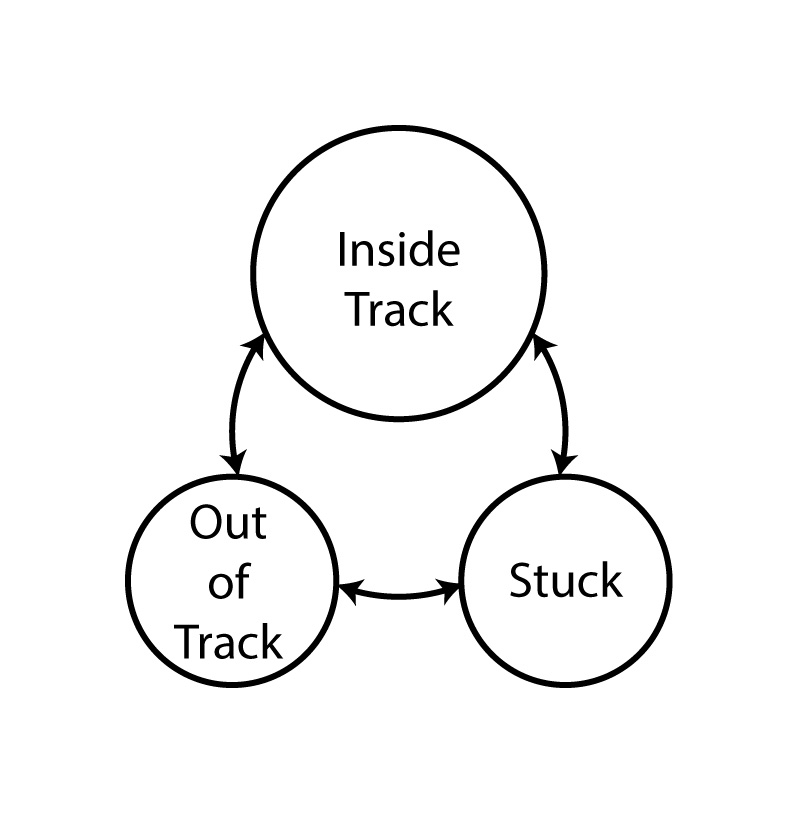
\includegraphics[width=.45\textwidth]{ThreeStateFSM}
	\caption{FSMDriver3 state diagram.}
	\label{Fig:FSM3Diagram}
\end{figure}

\IT~implements a very straightforward idea, get to an arbitrary target speed towards the largest open space inside track limits. The target speed is proportional to the largest sensor reading, and braking is activated if the current speed is greater than the target. Gear changing works based on RPM threshold as before. Overall, this implementation works for straight lines as well as curves.

In order to have a more detailed view of upcoming track segments the initialization of the range finders changed in the Three-State FSM. Here a normal distribution was applied in this intuit, focusing sensorial information ahead the car, as shown in Figure~\ref{Fig:FSM3Sensors}.
\begin{figure}[h]
	\centering
	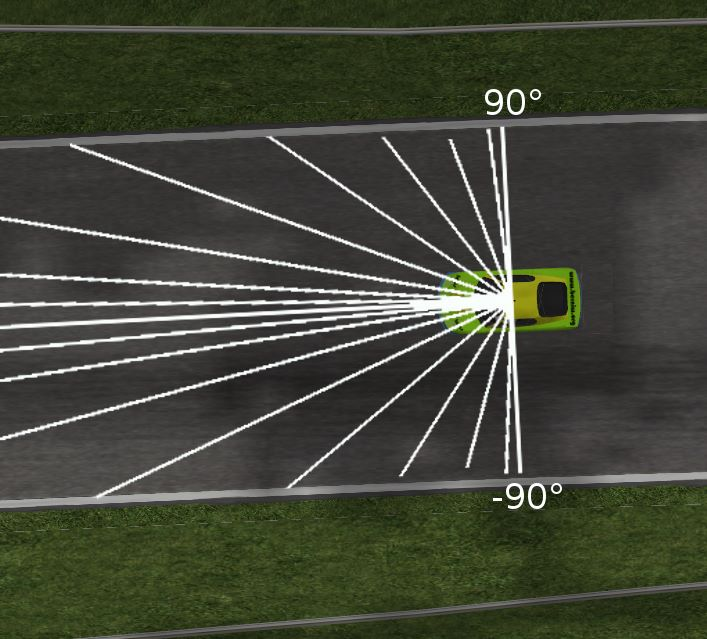
\includegraphics[width=250pt]{FSM3Sensors}
	\caption{FSMDriver3 range finders.}
	\label{Fig:FSM3Sensors}
\end{figure}

The transition function can then be reimplemented in a simpler fashion, as shown in Algorithm \ref{alg:FSMDriver3}:

\begin{algorithm}[h]%
\caption{FSMDriver3 Transition}%
\label{alg:FSMDriver3}%
\begin{algorithmic}
    \IF{car is stuck}
        \STATE $state \Leftarrow Stuck$
    \ELSE
        \IF{car is within track limits}
            \STATE $state \Leftarrow Inside Track$
        \ELSE
            \STATE $state \Leftarrow Out Of Track$
        \ENDIF
    \ENDIF
    \IF{the current state is not $state$}
        \STATE $Current State \Leftarrow state$
    \ENDIF
\end{algorithmic}
\end{algorithm}

Initially, configurations resembling FSMDriver5's parameters were set and manually adjusted until a behavior similar to the original driver was achieved. As expected, this process was quicker than for FSMDriver5 and soon a configuration better than some robots was available.

With the finished models\footnote{Code available at \url{https://github.com/bruno147/fsmdriver}}, the issue at hand became to set the models' parameter to such values as to maximize their performance, a large combinatorial problem to which a well known tool was applied.

\subsection{Evolving Parameters}%
In order to apply a genetic algorithm to the task of evolving the drivers' parameters, a model of the solution must be defined. In this context, a solution is called an individual and was represented by a string of bit parameters, that internally to the algorithm are interpreted as float numbers.

FSMDriver5 has, overall, 22 parameters from states and the transition function:

\begin{description}
	\item[Transition:] \ %
	\begin{description}
		\item[MAX\_STRAIGHTLINE\_VAR] upper boundary for classifying a straight line.
		\item[MIN\_STRAIGHTLINE\_VAR] lower boundary for classifying a straight line.
		\item[MAX\_APPROACHIN\_VAR] upper boundary for classifying an approaching curve.
		\item[MIN\_APPROACHIN\_VAR] lower boundary for classifying an approaching curve.
	\end{description}
	\item[Approaching Curve:] \ %
	\begin{description}
		\item[TARGET\_POS] desired percentage position.
		\item[BASE\_SPEED] lowest speed allowed during turns.
		\item[MAX\_STEERING] maximum allowed steering value.
	\end{description}
	\item[Straight Line:] \ %
	\begin{description}
		\item[LOW\_GEAR\_LIMIT] threshlod to bound low gears.
		\item[LOW\_RPM] threshlod of rpm to delimit the change of low gears.
		\item[AVERAGE\_RPM] threshlod to decrease high gears.
		\item[HIGH\_RPM] threshlod to delimit the change of high gears.
	\end{description}
	\item[Out of Track:] \ %
	\begin{description}
		\item[MAX\_SKIDDING] defines the threshold to start to break to avoid skidding.
		\item[NEGATIVE\_ACCEL\_PERCENT] dictate how much to release the acceleration pedal to avoid to skidding, its defined with the axis speed of car.
		\item[VELOCITY\_GEAR\_4] threshold to change the gear to 4.
		\item[VELOCITY\_GEAR\_3] threshold to change the gear to 3.
		\item[VELOCITY\_GEAR\_2] threshold to change the gear to 2.
		\item[MAX\_RETURN\_ANGLE] upper boundary to angle of return to track.
		\item[MIN\_RETURN\_ANGLE] lower boundary to angle of return to track.
	\end{description}
	\item[Stuck:] \ %
	\begin{description}
		\item[STUCK\_SPEED] defines the threshold to monitorate if its in stuck.
		\item[MINIMUM\_DISTANCE\_RACED] just to avoid to enter in stuck at the beginning of race when the car is stopped.
		\item[MAXIMUM\_NUMBER\_OF\_TICKS\_STUCK] maximum number of ticks in which reverse gear is allowed.
		\item[MAXIMUM\_NUMBER\_OF\_TICKS\_IN\_SLOW\_SPEED] maximum number of ticks in low speed before stuck is triggered.
	\end{description}
\end{description}

FSMDriver3, on the other hand, has the same 11 for \OT~and \St~ as FSMDriver5, plus 6 more:

\begin{description}
	\item[Inside Track:] \ %
	\begin{description}
		\item[LOW\_GEAR\_LIMIT] threshlod to bound low gears.
		\item[LOW\_RPM] threshlod of rpm to delimit the change of low gears.
		\item[AVERAGE\_RPM] threshlod to decrease high gears.
		\item[HIGH\_RPM] threshlod to increase high gears.
		\item[SPEED\_FACTOR] proportionality between highest value read by range finders and TARGET\_SPEED.
		\item[BASE\_SPEED] lowest speed allowed.
	\end{description}
\end{description}

The GA also requires a fitness function to evaluate the solutions, this work will consider the distance raced, which is also the standard metric for SCR.


%The first population was instantiated randomly to its full extent since there are no clues concerning how good an initial set of predefined parameters can be. This population passes through a fitness function that indexes a score to each individual, and this function is responsible for assessing how good - or how adapted - the solution that is being evaluated is. After evaluating the population, a group of individuals is chosen as the parents of the next set of solutions, which would compose a new generation; there are countless ways of performing the selection of the parents to the new generation of offspring, and this work gave preference to picking the higher individuals on the scoring system, what is called Elitism~\cite{ELITISM}. Each pair of parents was submitted to crossover in order to generate two offspring solutions, and in the end of the process each offspring might have presented mutation - everything according to predefined rates. The crossover took place in 95\% of the reproduction, while the mutation rate assumed the rate of 1\%~\cite{RATES}.
